\documentclass[a4paper, twocolumn, 12pt, twoside, english]{article}
\usepackage{geometry}
\geometry{verbose,tmargin=1in,bmargin=1in,lmargin=1in,rmargin=1in}
%\usepackage[utf8]{inputenc} % not used as we need ctex
%\usepackage[UTF8, scheme = plain]{ctex} %cjk is too old
%\usepackage[T1]{fontenc}
\usepackage{amsmath, amssymb, amsfonts, commath}
%\usepackage{lipsum}
%\usepackage{setspace}
%\usepackage{blindtext}
\usepackage{ulem}
\usepackage{subcaption}
\usepackage{graphicx}
\usepackage{stfloats}
\usepackage{wrapfig}
\usepackage{tcolorbox}


\author{Group 4\\Rui Gao\footnote{Corresponding author, garrygao@sjtu.edu.cn}\quad118370910003\\Guiwen Tan\quad118370910014\\ Muhammad Umer Siddique\quad118370990001\\Yu Cang\quad 018370210001}
\title{Wonder Builder: the first Skyscraper!}
\date{\today}

\begin{document}
\maketitle


\section{Introduction}
\begin{tcolorbox}[title = {Hello!}]
Welcome back to the time of inventions and rapid-development!

While the roars of steam whistle is still dominating the factories and rails, the second industrial revolution quietly started. With the invention of elevators, people start to look up for living space.

The time have come to conquer the sky!
\end{tcolorbox}

Welcome to {\it Wonder Builder: the first Skyscraper!}

You are the owner of a building company in the United States, the heart of the second industrial revolution. As a shrewd businessman, you are aware of the big chance hiding behind the invention of the elevators.

Construct a building that is higher than EVERY other building to draw the attention of the whole world. However, be aware that a lot of other businessmen are competing with you.

Fight through the difficulties and defeat other players, for the glory of building the first Skyscraper in the world!\bigskip

The goal of the game is to construct a skyscraper with toothpicks. To win, make sure that you are the first to build a 10-floor skyscraper. Both wisdom and luck are necessary to achieve final victory.


\section{Set Up the Game}

\subsection{Necessary Materials}
Some materials are needed before the game starts.

{\bf One table} with flat horizontal surface is needed to serve as the base for the buildings by the players.

{\bf Some toothpicks}\cite{ref:por} are needed as the construction material. A fair estimate for the total number of toothpicks needed is
\[
\text{Toothpicks Needed} \approx \text{No. Of Players} \times 50
\]

{\bf A dice} is needed to enable the game mechanics.

Figure~\ref{fig:stp} shows a typical setup.
\begin{figure}[!ht]
\centering
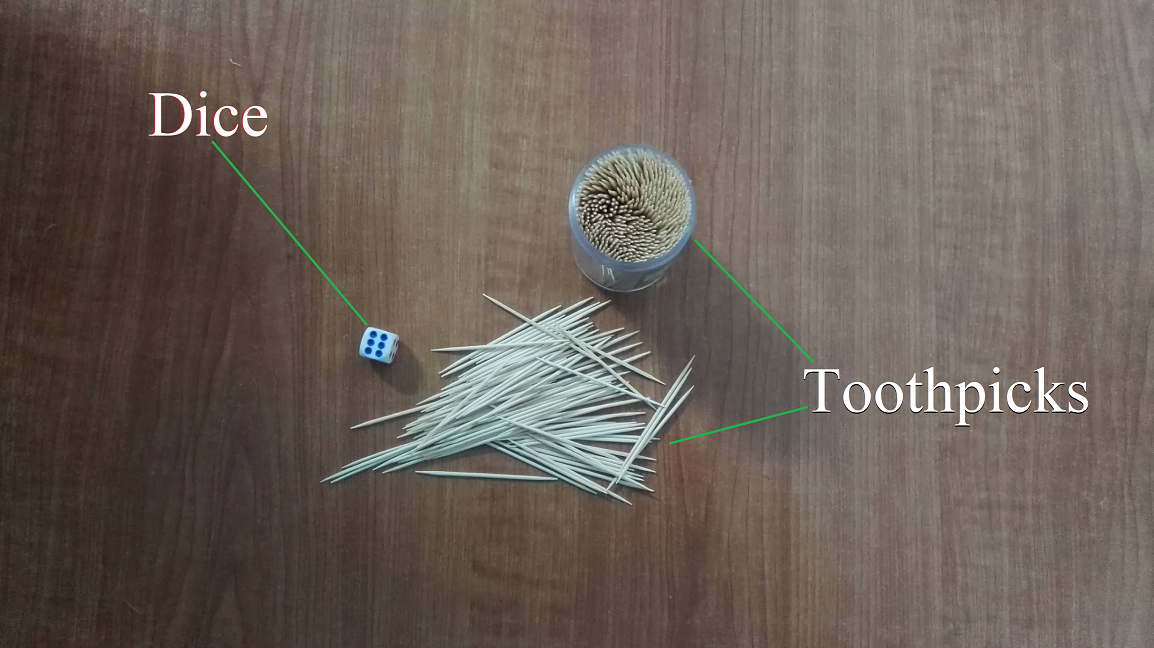
\includegraphics[width=0.45\textwidth]{Diagram_game_setup_2.png}
\caption{Necessary materials}
\label{fig:stp}
\end{figure}

\subsection{Start the Building}
\begin{tcolorbox}
You heard that a rival company has started to hire engineers and workers for their skyscraper. You decided to start immediately, but you need to find a suitable place to lay down the foundations.
\end{tcolorbox}
The players sit around the table. A random player starts his turn first, and then the next one clockwise starts his turn.

At the first turn, you need to throw a dice to see whether the place you selected is suitable. Throw six to lay the foundations of your building. If not, you need to re-throw next turn.

After a player has laid down the foundation, he could work on building surface floors in this turn and also later turns. See section~\ref{sec:turn} for detailed turn mechanics.


\subsection{End-Game Rules}
\begin{tcolorbox}
The Dutch are also planning to build a skyscraper. Obviously they will not stop to wait for you.
\end{tcolorbox}
The game concludes after 10 rounds, when Dutch people finished the famous {\it Witte Huis} in Rotterdam. The first player that finishes a 10-floor building before that wins the game.

\subsection{Build Proper Floors}
\begin{tcolorbox}
There was one stupid man in your hometown who one day erected a rod that is 10 stories high and claimed to have constructed a skyscraper. Everyone laughed at him.
\end{tcolorbox}
Similar to any other normal buildings, the surface of a floor should be flat. Figure~\ref{fig:flr} shows one of the correct and incorrect way to construct a two-floor building. The right building is not a correct two-floor building because the surface is not flat.
\begin{figure}[!h]
\centering
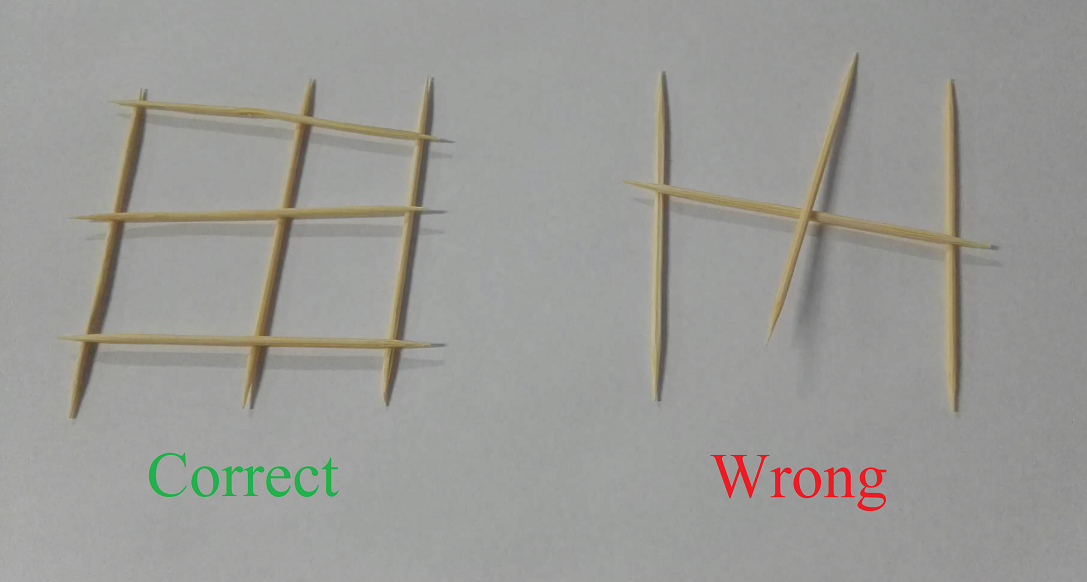
\includegraphics[width=0.45\textwidth]{Diagram_floors_2.png}
\caption{Correct and wrong examples of a two floor building}
\label{fig:flr}
\end{figure}

\section{Turn Mechanics}
\label{sec:turn}
Each turn is basically composed of two phases: Construction and Sabotage. In the Construction phase, the player constructs his building. In the Sabotage phase, the player attacks the buildings by other players. Figure~\ref{fig:flc} in the last page shows the flowchart if the game.
\subsection{Construction Phase}
\begin{tcolorbox}
To ensure the supply of building materials and fund, you go to bargain with the supplier and the bank, which would have random outcomes depending on your luck. Interestingly, the closer you are to success, the more helpful they become.
\end{tcolorbox}
In this phase, the player throws a dice to determine his supply of building material this turn, and additional toothpicks based on the current number of floors of his building. For example, if one that have a building of three floors throws five, then he would get three plus five toothpicks as his building material. The player can use these toothpicks to expand his existing building (or start to build one) in this turn. Each floor of the building can compose of any number of toothpicks as long as it does not collapse, but the player could only build on the topmost floor of the building, i.e., after the player starts to build the third floor, he cannot add toothpicks to the second floor anymore. Unused materials cannot be saved to the next turn.
%
%Version hand-sticking
%In this phase, the player sticks his hands to the toothpick container once to determine his supply of building material this turn. For example, if five toothpicks stick on his hands when he take his hands out, then he would get five toothpicks as his building material. The player can then use these toothpicks to expand his existing building (or start to build one if there is no building yet). Each floor of the building can compose of any number of toothpicks as long as it does not collapse, but the player could only build on the top floor of the building, i.e., after the player starts to build the second floor, he cannot add toothpicks to the first floor anymore. Unused materials cannot be saved to the next turn.
\subsection{Sabotage Phase}
\begin{tcolorbox}
``Business is war without bullets'', says Phil Knight. Some tricks may be helpful to your cause.
\end{tcolorbox}
In this phase, the player throws a dice. If the player throws five or six, then he successfully bribes one of the engineers in another company, and thus can sabotage another player's building by choosing one toothpick in his building and force the target player to remove that specific toothpick from the building.

If player A's building collapsed in player B's Sabotage phase, he enters the ``revival'' phase. See section~\ref{sec:rev} for details.

\subsection{Revival Phase}
\label{sec:rev}
\begin{tcolorbox}
``Failure the mother of success.'' You learn from the failure, and restart with better ideas in mind.
\end{tcolorbox}
Once a player's building collapsed, he enters the Revival phase. Depending on the reason for the collapse, he could restart his building effort with different terms.

If the building collapsed when the player is trying to build it, he should start from the ruins, i.e., what is left over after the collapse. For this turn and next turn only, he could build on any floor to strengthen the building.

If a player's building collapsed during another player's Sabotage phase, he should move to build a new building, as other parts of the old building may also be sabotaged. The player gains extra number of Construction phases equal to the number of floors left over in the ruin after the collapse. 

In either case, the revival phase lasts for two turns (the two active turns after the building collapsed), in which the player put all his focus on the rebuilding effort. The player could get construction materials using the same rule as the Construction phase, but he would not be able to sabotage other player's building during these two turns.

\begin{thebibliography}{}
\bibitem{ref:por}
Manuel Charlemagne, {\it Vg500 Technical Communication Project}. UM-SJTU JI canvas, available from https://umjicanvas.com/courses/962/ files/folder/project?

\end{thebibliography}
\newpage
\begin{figure*}
	\centering
	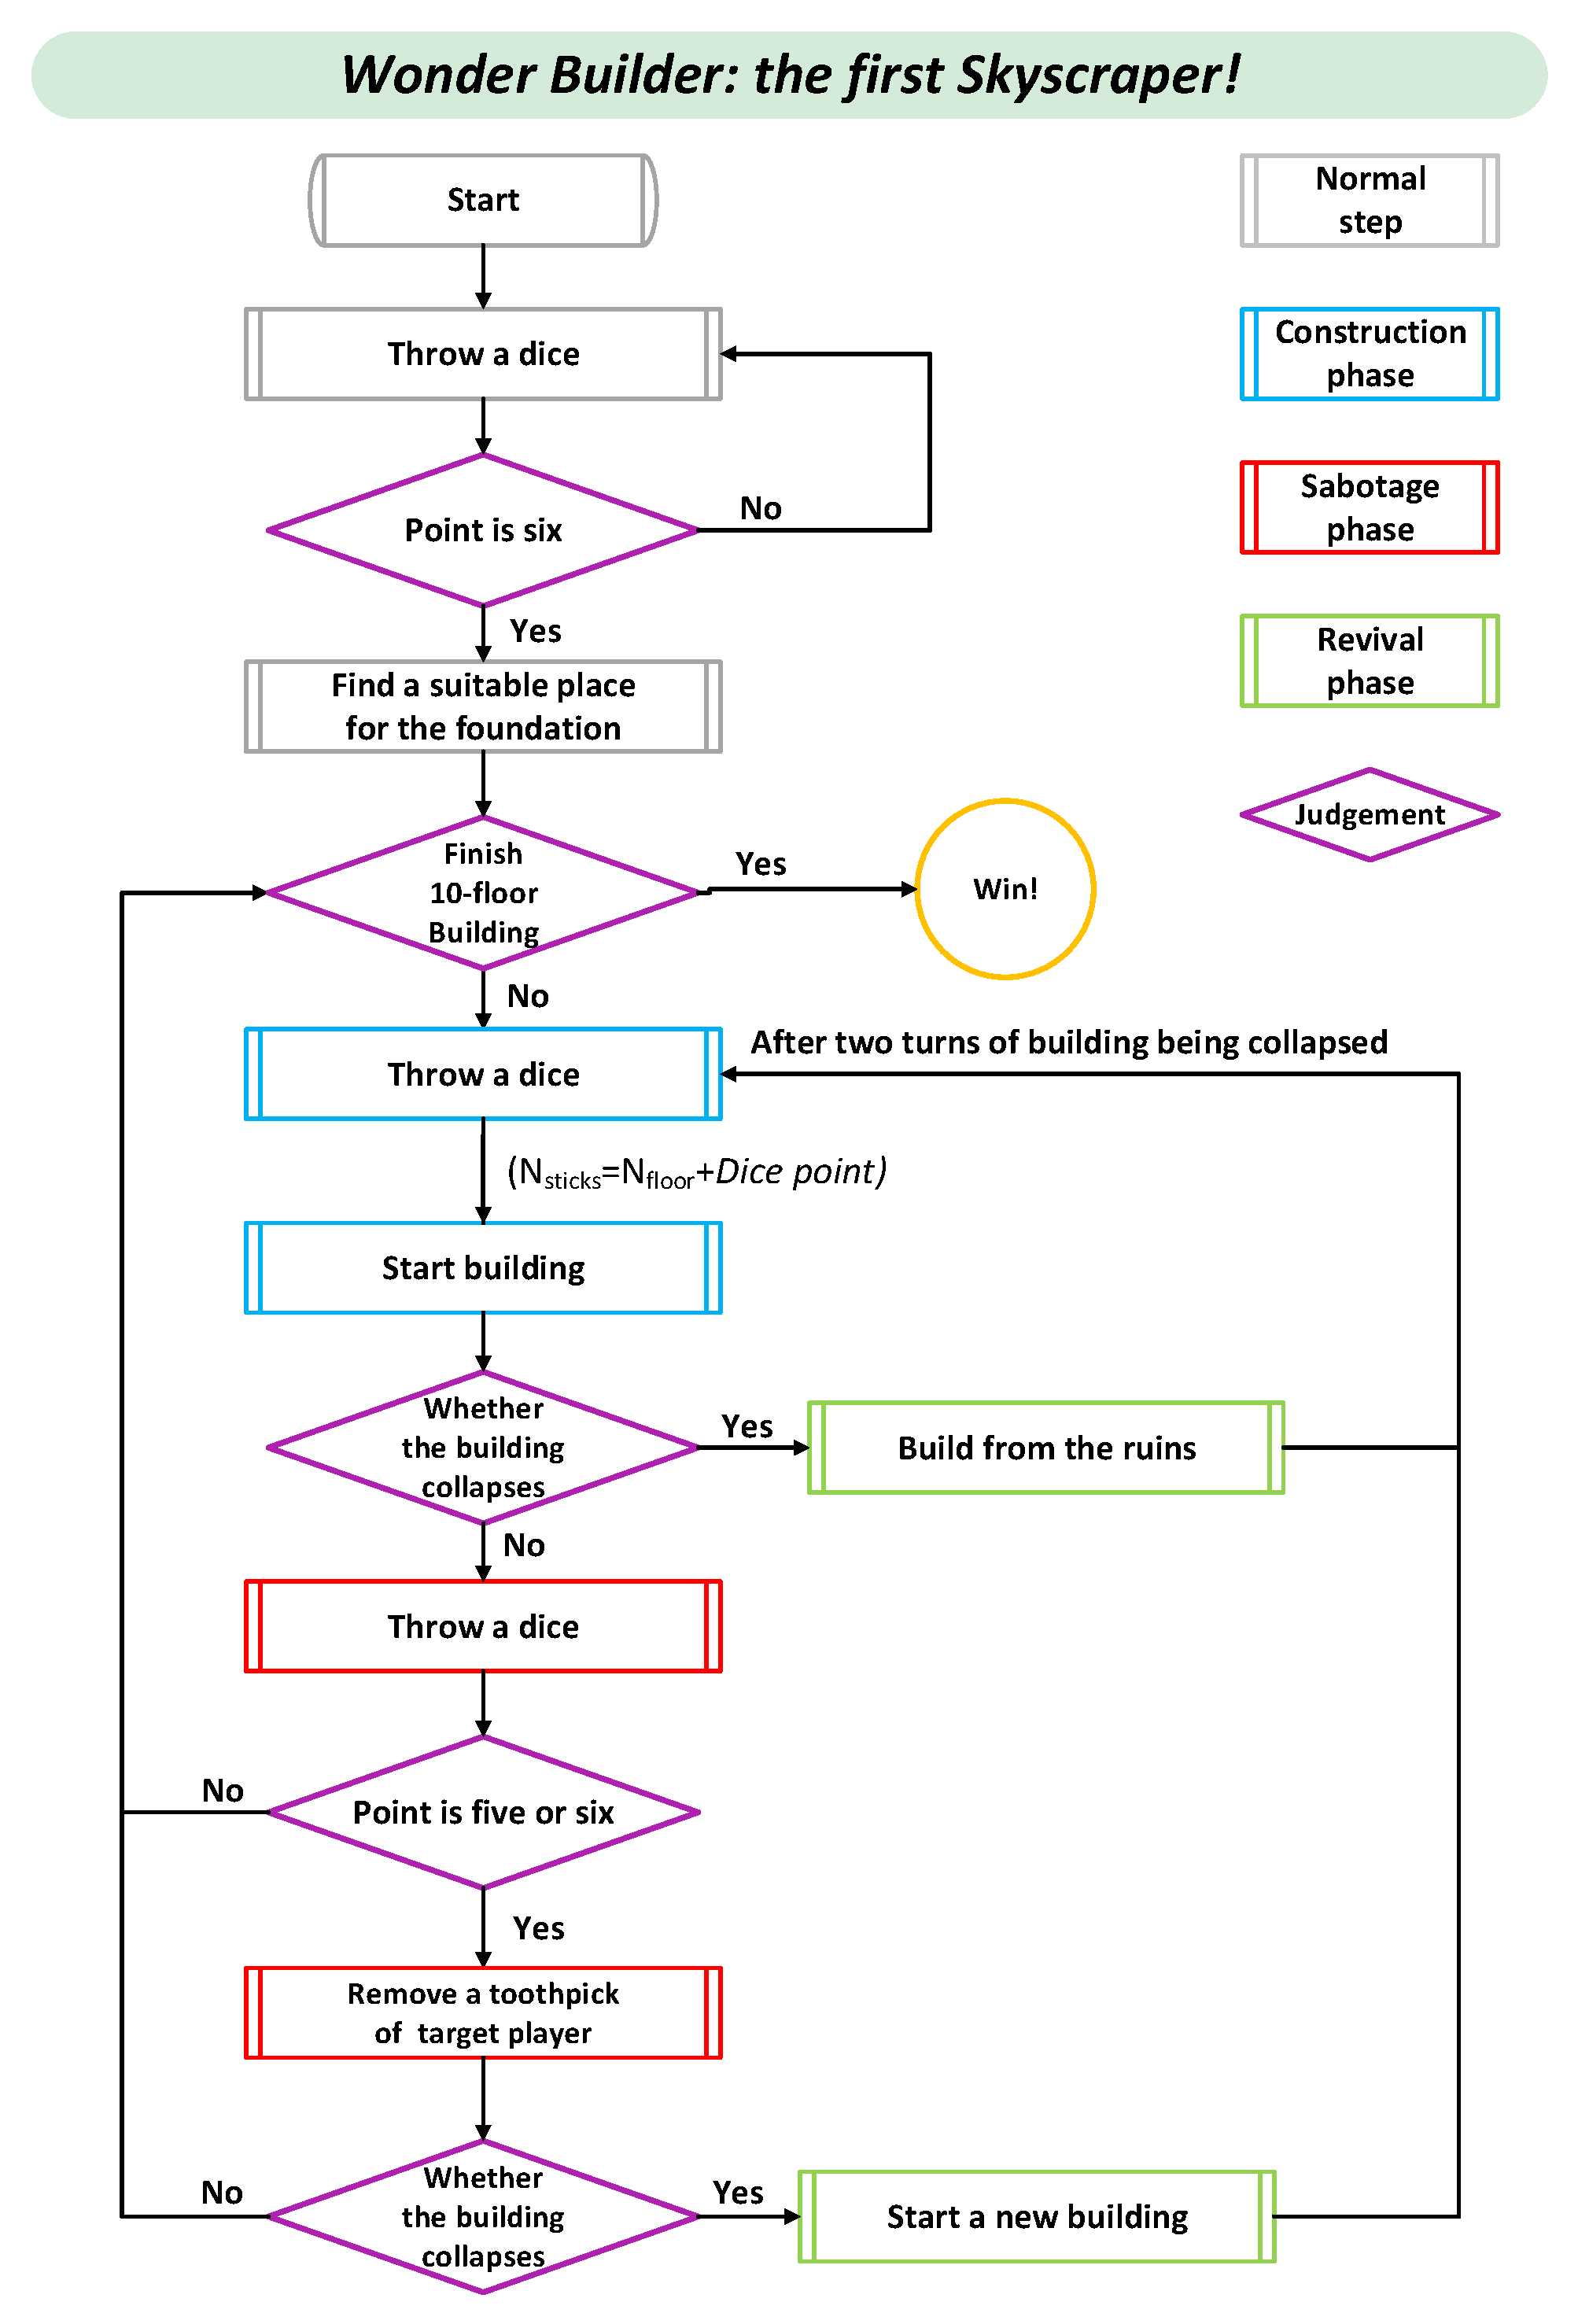
\includegraphics[width=1\textwidth]{flowchart.pdf}
	\caption{Flowchart for the game}
	\label{fig:flc}	
\end{figure*}
\end{document}
